
%%% Local Variables:
%%% mode: latex
%%% TeX-master: "../../doktorarbeit"
%%% End:

\chapter{Supernovae}
The history of supernovae starts, as most astrophysical objects, with observations of strong
electromagnetic events in the night sky. Supernovae are some of the most energetic events known to astronomers and throughout history, some have been clearly visible by naked eye from earth and could be seen even during the day (see \cite{hamacher_14} and references therein). 
The Crab supernova was in 1054 described by Chinese astronomers \citep{ho_96,shen_96}. 
\begin{displayquote}
\textit{... it was visible by day, like Venus; pointed rays shot out
from it on all sides; the color was reddish-white. Altogether it
was visible for 23 days.}
\end{displayquote}
\section{Classifying supernovae}
In the modern era observations of supernovae continually improved. In 1941
German-American astronomer Rudolph Minkowski \citep{minkowski_41} found
that not all supernovae show hydrogen lines in their spectra and
he consequently divided supernovae into two types based on the
presence of hydrogen (Type II) or lack of hydrogen lines (Type I).
Later it was recognized that there were variations within these two classes
and a set of subclasses, based on variation in the spectra and light curve. 
Type I supernovae were divided into type Ia, Ib, and Ic,
where the nebular spectrum of types Ib and Ic was found to be similar to
those of type II supernovae. Two examples of the type II sub-classes are
types II-L and II-P. After reaching the maximum luminosity, the light curves of type II-P supernovae settles onto a
plateau and their luminosity reminds almost constant for several months. The luminosity of Type II-L, on the other hand, 
decline almost linearly. For a detailed review of the classification system see \cite{cappellaro_01}.

The similarities between the nebular spectra of type II and type Ib/c supernovae already hints at a similar explosion mechanism. From a theoretical standpoint, one might say that a classification based on physical processes
powering the supernovae is more prudent. Already in 1960 \cite{hoyle_60} suggested that type II supernovae result from
the implosion of stellar cores and that type I is produced by igniting degenerate stellar material. Today it is understood that
that type Ia supernovae result from the thermonuclear explosions of white dwarfs. In other words, the ignition of degenerate stellar material.
Furthermore, we now know that type II and type Ib/c supernovae are the result of the gravitational collapse, the implosion, of stellar cores.
The latter category are known as core-collapse supernovae. The subject of this thesis is the gravitational waves generated during the collapse and subsequent explosion of a specific sub-type of core-collapse supernova, the ``Iron-core supernova'', and we, therefore, 
constrain our attention to this class of supernovae. The interested reader is referred to \cite{janka_12} for a comprehensive description of the possible explosion mechanisms.

\section{Iron-core supernovae}
\subsection{Shell burning in massive stars}
\begin{wrapfigure}{r}{0.5\textwidth}
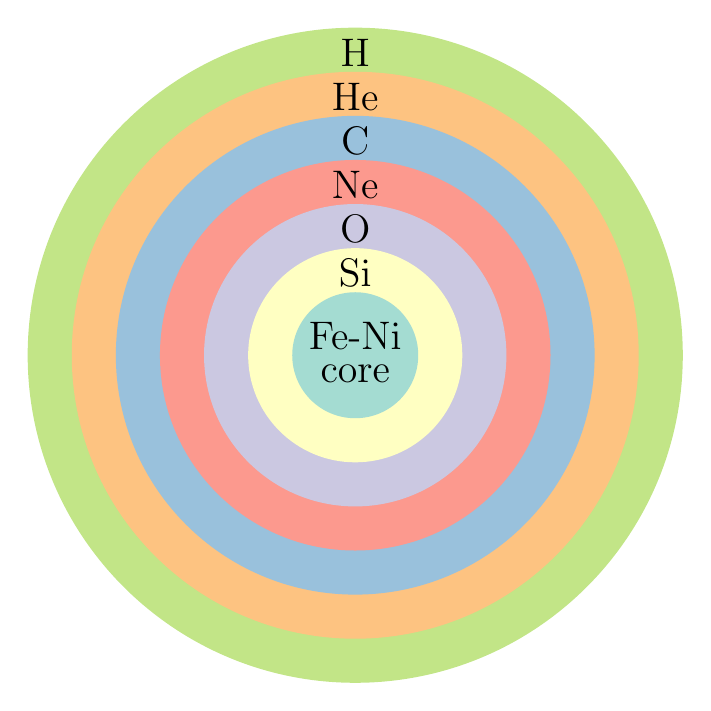
\begin{tikzpicture}[scale=0.8]
\definecolor{c1}{RGB}{141,211,199}
\definecolor{c2}{RGB}{255,255,179}
\definecolor{c3}{RGB}{190,186,218}
\definecolor{c4}{RGB}{251,128,114}
\definecolor{c5}{RGB}{128,177,211}
\definecolor{c6}{RGB}{253,180,98}
\definecolor{c7}{RGB}{179,222,105}
\fill[c7!80] (0,0) circle (5.2cm);
\fill[c6!80] (0,0) circle (4.5cm);
\fill[c5!80] (0,0) circle (3.8cm);
\fill[c4!80] (0,0) circle (3.1cm);
\fill[c3!80] (0,0) circle (2.4cm);
\fill[c2!80] (0,0) circle (1.7cm);
\fill[c1!80] (0,0) circle (1cm);
\node at (0,0.3) {\Large{Fe-Ni}};
\node at (0,-0.3) {\Large{core}};
\node at (0,1.3) {\Large{Si}};
\node at (0,2.) {\Large{O}};
\node at (0,2.7) {\Large{Ne}};
\node at (0,3.4) {\Large{C}};
\node at (0,4.1) {\Large{He}};
\node at (0,4.8) {\Large{H}};
\end{tikzpicture}
\caption{Schematic representation of the shell structure of a massive star right before
the onset of core-collapse. The stellar core consists of consecutive layers burning heavier
and heavier elements and an inner iron-nickel core.}
 \label{figSN:onion}
\end{wrapfigure}
When a massive star nears the end of its life it has depleted most of the hydrogen in the central core
and hydrogen burning ceases and the gravitational pull is no longer balanced by thermal and radiation pressure resulting
from nuclear fusion. The consequence is that the core starts to contract, the contraction is eventually halted when the pressure
and temperature in the core become large enough for helium burning to set in. The layer right outside of the helium burning core is still rich
in hydrogen and so hydrogen burning develops in a layer around the core. The burning of helium in the core stabilises the star, for a while.
However, the helium fuel eventually runs out and the process repeats itself, only this time the contraction continues until carbon ignites in the inner core. 

The process of burning heavier and heavier elements in the core continues up to silicon. The end product of silicon burning is iron-group elements and
since nuclear fusion of iron-group elements does not release any energy the cycle stops at silicon. The end result of this process is
an onion like shell structure consisting of consecutive layers burning heavier and heavier elements. In the centre of this onion is ever growing
core consisting of iron and nickel (henceforth referred to as the ``iron-core''), it grows due to the ashes produced by the continued burning of silicon in the layer above. A depiction of this shell structure can be seen in \fig{figSN:onion}.
The star remains in this state for a while,
until the central iron-core has accumulated so much matter that its mass exceeds the Chandrasekhar mass and the inevitable gravitational collapse 
of the core begins.
% As John Connor, the star has no hopes of stopping judgement day, it can only hope to postpone it. 
% Gravitational collapse is, as the terminator puts it, inevitable.

\subsection{Iron-core collapse}
The collapse of the iron-core is triggered and accelerated by two processes.
Firstly, rising temperatures increase the rate of photo-dissociation of iron-group 
nuclei. The nuclei are converted into free nucleons and alpha particles,
which is a process that consumes thermal energy. Secondly, as the core density increases electron capture
on heavy nuclei becomes more frequent. Free electrons are capture by protons in the nuclei and a neutrons 
and anti-electron neutrinos are produced:
\begin{equation} \label{eqSN:ecapture}
p + e^{-} \rightarrow n + \bar{\nu}_e,
\end{equation}
where $p^{+}$, $e^{-}$, $n$ and $\bar{\nu}_e$ represents a proton, an electron, 
a neutron and an anti-electron neutrino, respectively.
The neutrinos escape the core and in the process carry with them energy
and lepton number. Before the onset of collapse it was pressure from degenerate electrons
that was suporting the core. Whent he lepton number decreases the this pressure also decreases,
and this leads to an acceleration of the collapse. Effectively what is happening is that
the Chandrasekhar mass of the core is reduced. 

The rapid deleptonisation of the iron-core eventually slows down and virtualy stops for the duration of the collapse. 
At densities around $10^{12}$ g/cm$^3$ the mean free path of the neutrinos become so short that the time they need to diffuse out of the
core is larger than the time-scale of the collapse. The iron-core, therefore, from this point on collapses in an 
adiabatic and homologous manner. The collapse continues until the central iron-core reaches nuclear densities, around $2.7 \times 10^{14} $g/cm$^3$,
at this point the repulsive forces between nuclei leads to a sudden stiffening of the equation of state (EoS) and the collapse of the
inner iron-core comes to an abrupt halt. 

However, due to its high inertia the inner core contracts beyond the equilibrium point of the
gravitational pull and the new source of pressure. This leads to a recoil and as the inner region of the iron-core expands outwards it crashes
into the infalling material above it. This event is the so-called core bounce and it launches a sound wave into the outer iron-core, that steepens into a shock wave when it reaches the supersonically infalling layers of the outer core.

As the shock propagates outwards through the dense stellar material it looses about 
$10^{51}$ erg of energy per 0.1 \msun of iron-core material that falls through the shock front, 
due to the dissociation of heavy nuclei into free nucleons.
Eventually, the density ahead of the shock drops below $\sim \, 10^{11}$ g/cm$^3$ and
the neutrinos behind the shock can suddenly escape. This leads to a burst of neutrino emission and a significant loss of energy for the shock. After a few milliseconds (ms) the
shock has lost so much energy that it stalls at a radius between 100 and 200 km
and turns into an accretion shock.

\subsection{Shock revival: the neutrino heating mechanism}
It was initially thought that the shock would not stall, but rather propagate
throughout the mantle of the star and disrupt it in the process. 
This mechanism is known as the bounce-shock or prompt-shock mechanism.
As mentioned above, the shock only propagates outwards a for a few ms before losing most of its
energy and stagnating. The failure of the bonce-shock mechanism
can be viewed as a consequence of its failure to account for anything else than purely hydrodynamical effects. Most of the gravitational binding energy released during the collapse is stored in
the form of trapped neutrinos and tapping into this energy reservoir might provide the energy needed to revive the stalled shock.
Already in 1966 \cite{colgate_66} proposed that neutrinos cold be the principle
actor in the drama unfolding deep within the star. Later this idea was revisited and expanded upon by \cite{wilson_85}
who formulated the so-called ``delayed neutrino-driven explosion mechanism''.

At the same time as the shock is initially launched a hot proto-neutron star (PNS)
forms in the center of the star. The gravitational binding energy released during the collapse is 
converted into thermal energy. The PNS mainly cools
through emission of neutrinos, which first slowly diffuse through the optically thick inner-core
before breaking out of the so-called neutrinosphere and streaming away from the core.
The neutrinosphere is defined by the radius where the core becomes optically thin to neutrinos.
A secondary source of neutrinos is the matter falling through the stalled shock and accreting onto the PNS, 
which releases neutrinos as the material settles onto the PNS. The catpure of electrons and positrons 
on free nucli is the main source of neutrinos in the hot accretion layer
around the PNS. This means that electron and anti-electron neutrinos makes up 
a large fraction of the neutrino emission generated by PNS accreation. 

The material falling through the
shock also exerts the ram pressure that must somehow be counteracted to relaunch the shock.
As neutrinos stream away from the core a small fraction of their energy is deposited into the
stellar material behind the shock, because this material is not perfectly optically thin to neutrinos.
It is this energy deposition that is thought to balance and eventually overcome the ram pressure of the infalling of the material, leading to the successful
revival of the stalled shock.

\section{The post-bounce phase}
The phase between core bounce and shock revival is a crucial time period for the delayed neutrino-driven explosion mechanism. 
The focus of this thesis is to study what we can learn about core collapse supernovae
by observing the gravitational wave (GW) signal they produce. Specifically this work focuses on
fingerprints of hydrodynamical processes operating during the post-bounce phase. 
In this section we discuss our current understanding of the properties of the region behind
the stalled shock front, consisting of the PNS and the region between the PNS and the shock front (known as the post-shock volume/region/layer). 

\subsection{The gain layer, cooling layer and the three layers of the Proto-neutron star}
The fact that the mean free path of the neutrinos increases with radius means that
neutrino diffusion more effectively carries away lepton number and entropy in the 
outer regions of the PNS core. This leads to the establishment of negative 
entropy and composition gradients, which in turn creats a convectivly unstable 
region located between the surface and the inner PNS core (see \fig{figSN:post}).

The heating of the stellar material in the post-shock region is dominated by charged-current reactions
\begin{align} \label{eqSN:heat}
n+ \nu_e & \rightarrow p + e^{-}, \nonumber \\
p + \bar{\nu}_e& \rightarrow n + e^{+},
\end{align}
and cooling by the corresponding inverse interactions
\begin{align} \label{eqSN:cool}
p + e^{-} & \rightarrow n+ \nu_e , \nonumber \\
n + e^{+}  & \rightarrow p + \bar{\nu}_e.
\end{align}
\begin{figure}%{r}{0.6\textwidth} 
\begin{center}
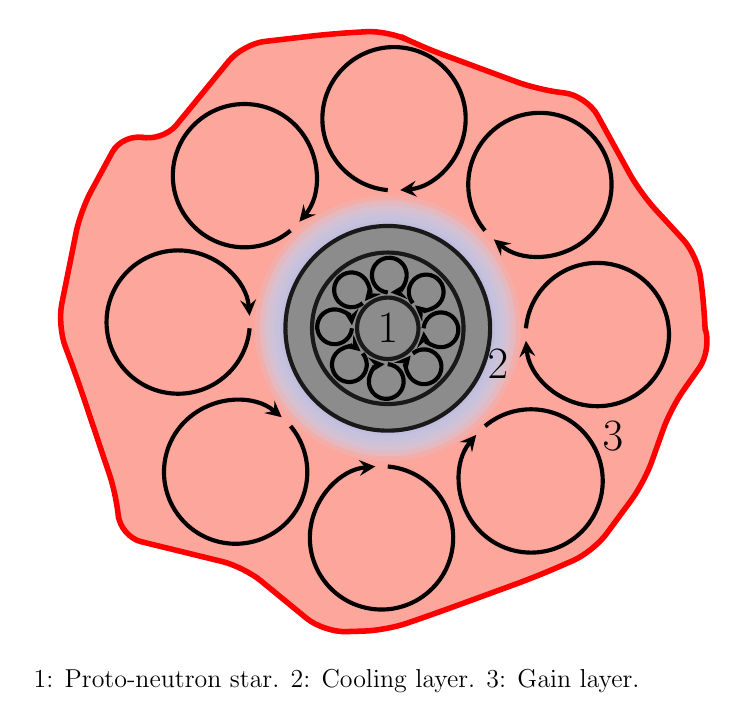
\begin{tikzpicture}[scale=0.65, every node/.style={scale=0.65},decoration={random steps,segment length=1cm,amplitude=.42cm,pre=lineto,pre length=.25cm,post=lineto,post length=.25cm}]
\definecolor{c3}{RGB}{190,186,218}
\definecolor{c4}{RGB}{251,128,114}
\draw[red,decorate,rounded corners=7.90pt,line width=2pt,fill=c4!70] (0,0) ellipse (6.2cm and 5.7cm);
\fill[c3,line width=1.5pt] (0,0) circle (2.cm);

\fill[c3!70,line width=1.5pt,opacity=0.2] (0,0) circle (2.6cm);
\fill[c3!75,line width=1.5pt,opacity=0.4] (0,0) circle (2.5cm);
\fill[c3!80,line width=1.5pt,opacity=0.5] (0,0) circle (2.4cm);
\fill[c3!85,line width=1.5pt,opacity=0.6] (0,0) circle (2.3cm);
\fill[c3!90,line width=1.5pt,opacity=0.8] (0,0) circle (2.2cm);
\fill[c3!95,line width=1.5pt,opacity=1.] (0,0) circle (2.1cm);

\fill[gray!90] (0,0) circle (2.cm);
\draw[black!90,line width=1.5pt] (0,0) circle (2*.74cm);
\draw[black!90,line width=1.5pt] (0,0) circle (.6cm);
\draw[black!90,line width=1.5pt] (0,0) circle (2.cm);

\draw [>=stealth,->, line width=1.5pt,rotate=0] (2.7,0) arc (175:-175:1.4cm);
\draw [>=stealth,->, line width=1.5pt,rotate around={180:(-2.7,0)}] (-2.7,0) arc (175:-175:1.4cm);
\draw [>=stealth,->, line width=1.5pt,rotate around={90:(0,2.7)}] (0,2.7) arc (175:-175:1.4cm);
\draw [>=stealth,->, line width=1.5pt,rotate around={-90:(0,-2.7)}] (0,-2.7) arc (175:-175:1.4cm);
\draw [>=stealth,->, line width=1.5pt,rotate around={45:(1.9,1.91)}] (1.9,1.91) arc (175:-175:1.4cm);
\draw [>=stealth,->, line width=1.5pt,rotate around={-45:(1.9,-1.91)}] (1.9,-1.91) arc (175:-175:1.4cm);
\draw [>=stealth,->, line width=1.5pt,rotate around={-135:(-1.9,-1.91)}] (-1.9,-1.91) arc (175:-175:1.4cm);
\draw [>=stealth,->, line width=1.5pt,rotate around={135:(-1.9,1.91)}] (-1.9,1.91) arc (175:-175:1.4cm);

\draw [>=stealth,->, line width=1.5pt,rotate=0] (.7,0) arc (175:-175:.34cm);
\draw [>=stealth,->, line width=1.5pt,rotate around={180:(-.7,0)}] (-.7,0) arc (175:-175:.34cm);
\draw [>=stealth,->, line width=1.5pt,rotate around={90:(0,.7)}] (0,.7) arc (175:-175:.34cm);
\draw [>=stealth,->, line width=1.5pt,rotate around={-90:(0,-.7)}] (0,-.7) arc (175:-175:.34cm);
\draw [>=stealth,->, line width=1.5pt,rotate around={45:(.49,.491)}] (.49,.491) arc (175:-175:.34cm);
\draw [>=stealth,->, line width=1.5pt,rotate around={-45:(.49,-.491)}] (.49,-.491) arc (175:-175:.34cm);
\draw [>=stealth,->, line width=1.5pt,rotate around={-135:(-.49,-.491)}] (-.49,-.491) arc (175:-175:.34cm);
\draw [>=stealth,->, line width=1.5pt,rotate around={135:(-.49,.491)}] (-.49,.491) arc (175:-175:.34cm);
\node at (0,0) {\Huge{1}};
\node at (2.15,-0.7) {\Huge{2}};
\node at (2*2.2,-3*0.7) {\Huge{3}};
\node[align=left] at (-1,-6.9) {\Large{1: Proto-neutron star.} \Large{2: Cooling layer.} \Large{3: Gain layer.}};
\end{tikzpicture}
\end{center}
\caption{Schematic representation of the region behind the shock. The grey region indicates the PNS, the light blue
region shows the cooling layer and the gain layer is indicated by the light red region. The dark red boundary shows the shock
front with its large and small scale deformations. Circular arrows indicate the two regions that are convectively active. }
\label{figSN:post}
\end{figure}
The neutrino-cooling rate, caused by the reactions described by \eq{eqSN:cool}, depends on the temperature to the sixth power, $\sim \, T^6$. 
Since the temperature of the convectively mixed 
post-shock layer drops roughly as $\sim \, 1/r$ \citep{janka_12} the cooling efficiency drops as $\sim \, r^{-6}$  
The heating rate, on the other hand, drops off only as radius squared, $\sim r^{-2}$.     
As a result, there exists a radius where heating and cooling effects balance each other.
This radius is called the ``gain radius''. Below the gain radius neutrino cooling dominates
and above there is a net heating by neutrinos. The neutrino heating from below makes the gain layer unstable to
large scale convective activity. The high-entropy bubbles that are created by convection in
pushes shock front outwards. This prolongs the time it takes for stellar matter to be advected through the layer, which enhances the heating done by neutrinos. 
Convection also transports heated material away from the gain radius and prevents it from falling down into
the cooling layer. The end result is that the matter falling through the shock spends considerably more time
in the gain layer than it would without the development of convection.
This favours the delayed neutrino-driven explosion mechanism and has been studied by several authors
(see for example \cite{herant_94,burrows_95,janka_96,foglizzo_06,mueller_12a}).
In \fig{figSN:post} we see a schematic depiction, not to scale, of
the region behind the stalled shock. The PNS is indicated by the grey region, the cooling layer by the light blue and
the light red region indicates the gain layer. The circles with arrows indicate convection. The dark red curve
at the edge of the gain layer indicates the shock front, with its large and small scale deformations.

\subsection{The standing accretion shock instability}
Another instability that can develop and be beneficial for the explosion mechanism is 
the so-called standing accretion shock instability (SASI), which manifests itself in large-scale 
sloshing and spiral motions of the shock \citep{blondin_03,blondin_06,foglizzo_07,ohnishi_06,ohnishi_08,scheck_08,guilet_12,foglizzo_15}.
The SASI develops through an advective-acoustic cycle, entropy and vorticity perturbations from the shock are advected through the
post-shock layer and when they are decelerated at the PNS surface they are converted into pressure waves that propagate
out towards the shock front. Once these acoustic waves hit the stalled shock they perturb it, completing the feedback
cycle. The large-scale deformation of the shock pushes the average radius outwards and therefore enhances neutrino heating.
 
\section{Three-dimensional simulations}
After promising results from 
two-dimensional (2D) simulations supernova modelers experienced initial setbacks in three-dimensional (3D) \citep{hanke_12,hanke_13}.
Now, however, we are starting to see the emergence of the first generation
of successful 3D simulations of explosions with three-flavour
multi-group neutrino transport, culminating in the recent models
of the Garching and Oak~Ridge groups
\citep{melson_15a,melson_15b,lentz_15} with their rigorous treatment
of the transport and neutrino microphysics in addition to many more
obtained with more approximate transport schemes,
as for example the studies of \citet{takiwaki_12,takiwaki_14}, 
\citet{mueller_15b} and \citet{roberts_16}.
\citet{takiwaki_12,takiwaki_14} employ the isotropic diffusion source 
approximation \citep{liebendoerfer_09}
and use further approximations to treat heavy lepton neutrinos.
\cite{takiwaki_14} employ a leakage scheme to account for heavy lepton
neutrinos and \cite{takiwaki_12} neglect the effect of these neutrinos 
altogether. \cite{mueller_15b} utilises the stationary fast multi-group 
transport scheme of \cite{mueller_15a}, which 
solves the Boltzmann equation at high optical depths in a two-stream approximation and
matches the solution to an analytic variable 
Eddington factor closure at low optical depths.
\citet{roberts_16} employ a full 3D two-moment (M1) solver in 
general relativistic simulations, but ignore velocity-dependent
terms.
On the other hand, it has proven difficult to consistently 
relaunch the stalled supernova shock in full 3D simulations.
Numerical modeling of core-supernovae is an active field of
research and as of now there is no consensus of what exactly 
is the key to successful 3D explosions.

